
\item A tennis ball is dropped on a horizontal smooth surface. It bounces back to its original position after hitting the surface. The force on the ball during the collision is proportional to the length of compression of the ball. Which one of the following sketches describes the variation of its kinetic energy \( K \) with time\( t \) most appropriately? The figures are only illustrative and not to the scale.
    \begin{tasks}(2)
        \task 
        \begin{center}
            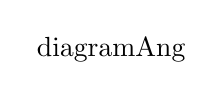
\begin{tikzpicture}
                \node at (0, 0) {diagramAng};
            \end{tikzpicture}
        \end{center}
        \task 
        \begin{center}
            
\begin{tikzpicture}
                \node at (0, 0) {diagramBpng};
            \end{tikzpicture}
        \end{center}
        \task 
        \begin{center}
            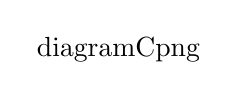
\begin{tikzpicture}
                \node at (0, 0) {diagramCpng};
            \end{tikzpicture}
        \end{center}
        \task 
        \begin{center}
            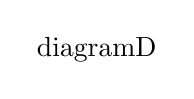
\begin{tikzpicture}
                \node at (0, 0) {diagramD};
            \end{tikzpicture}
        \end{center}
    \end{tasks}
